\documentclass[9pt]{article}

\usepackage[latin1]{inputenc}
\usepackage[T1]{fontenc}
\usepackage{ngerman}
\usepackage{fancyhdr}
\usepackage{graphicx}

\pagestyle{fancy}

\setlength{\headheight}{60pt}
\lhead[]{\Large{\textbf{Verteilte Systeme 2012: Zusammenfassung}} \\}

\begin{document}
\section{Systemarchitekturen nach Flynn}
\subsection{SISD (Von-Neumann-Architektur)}
Single Instruction Single Data \\
ein Instruktionsstrom und ein Datenstrom \\
sequentielle Uniprozessorarchitektur, ggf. aber interne Parallelit�t durch Pipelining oder intelligente I/O-Kan�le

\subsection{SIMD}
Single Instruction Multiple Data \\
ein Instruktionsstrom, mehrere Datenstr�me \\
Beispiele: Vektorprozessoren, Grafikkarten \\
Ausblenden einzelner Prozessoren durch Tagging m�glich $\leftarrow$ Prozessoren k�nnen simultan verschiedene Operationen ausf�hren

\subsection{MIMD}
Multiple Instruction Multiple Data \\
Systeme mit \begin{itemize}
\item gemeinsamem Speicher ("`shared memory"', SMP)
\item verteiltem Speicher ("`distributed memory"', DMS)
\end{itemize}
Prozessoren werden �ber Verbindungsnetzwerk gekoppelt, jeder wird �ber einen unabh�ngigen Instruktionsstrom gesteuert \\
Prozessoren arbeiten autonom und haben �ber Verbindungsnetzwerk Zugriff auf die Daten der anderen Prozessoren 

\subsection{MISD}
Multiple Instruction Single Data \\
Eher nicht verwendet, als Beispiel aber FPGA

\section{SPMD - Single Program, Multiple Data}
\textbf{nicht Teil der Flynn-Taxomonie} \\
Grundprinzip: Alle (MIMD-)Prozessoren arbeiten auf Kopien desselben Programmcodes, aber mit unterschiedlichen Daten und ggf. in
unterschiedlichen Modulen. \\
Vorteile \begin{itemize}
\item leichte Programmentwicklung, -debugging, -wartung
\item leichtere Synchronisation als "`echte"' MIMD-Programmierung
\item gr�bere Parallelit�tsgranularit�t als SIMD
\end{itemize}

\section{Verteilte Systeme allgemein}
\subsection{Definition}
Menge miteinander verbundener, autonomer Computer, die dem Nutzer wie ein einzelnes koh�rentes System erscheinen.
\begin{itemize}
\item "`Computer"': Prozessoren/Prozesse
\item "`autonom"' : jeder Knoten hat private Kontrolle (kein SIMD)
\item "`miteinander verbunden"' : Informationsaustausch ist m�glich
\end{itemize}

Typen: \begin{itemize}
\item Computer in WANs - Internet, Intranet
\item Computer im LAN - Hausnetz einer Universit�t
\item kooperierende Prozesse/Threads - Prozesse und Threads auf einer Maschine
\end{itemize}

\subsection{Vorteile/Motivation}
\begin{itemize}
\item Informationsaustausch
\item Zuverl�ssigkeit durch Replikation
\item Ressourcensharing (Drucker, Festplattenspeicher, Rechenleistung)
\item Leistungssteigerung durch Parallelisierung
\item Vereinfachung des Systemdesigns durch Entkopplung/Spezialisierung
\end{itemize}

\subsection{Anforderungen}
\begin{itemize}
\item Transparenz - Verteilung bleibt dem Benutzer verborgen
\item Offenheit - Austausch und Erweiterbarkeit (von Komponenten)
\item Skalierbarkeit - gleich gute Leistung unabh�ngig von der Nutzeranzahl 
	\begin{itemize}
	\item Gr��e - mehr Nutzer und Ressourcen
	\item geographische Verteilung
	\item administrativ - �ber Organisationsgrenzen hinweg administrierbar
	\end{itemize}
\end{itemize}
Realisierung von Transparenz durch Middleware: \\
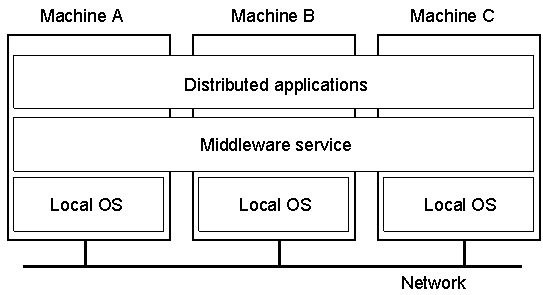
\includegraphics[width=80mm]{verteiltesSystemBeispiel.png}
\section{Parallele Programmierung}
\subsection{Betriebssystemsicht}
\begin{itemize}
\item Multicomputerbetriebssystem: erbringt die Systemdienste verteilt und transparent
	\begin{itemize}
	\item pr�sentiert dem Nutzer ein koh�rentes System
	\item hat vollst�ndige Kontrolle �ber Knoten und deren Ressourcen
	\item kann keine heterogenen Systeme verwalten
	\end{itemize}
\item Netzwerk-Betriebssystem: erlaubt, Dienste entfernt zu nutzen, bietet aber keine Transparenz
	\begin{itemize}
	\item verteilte Rechner mit autonomen Betriebssystemen und eigener Ressourcenverwaltung
	\item eingebaute Netzwerkfunktionalit�t
	\item skalierbar und offen
	\end{itemize}
\end{itemize}
Middleware: \begin{itemize}
\item bietet Abstraktionen f�r Netzwerkprogrammierung $\leftarrow$ \textbf{bessere Transparenz}
\item bietet relativ kompletten Satz von Diensten
\item Event Handling und Filtering
\item Auffinden von Ressourcen f�r mobiles Computing
\item Unterst�tzen von Datenstr�men
\end{itemize}

\subsection{Parallele Programmierung}
Ausgewogenes System: Forderung pro Operation/s:
\begin{itemize}
\item 1 Byte Hauptspeicherkapazit�t
\item 100 Byte Plattenspeicher
\item 1 Bit I/O-Rate
\end{itemize}

Leistungssteigerung durch:
\begin{itemize}
\item Pipelining: mehr Instruktionen pro Zeit durch parallel arbeitende Funktionale Einheiten
\item Superscalar: mehr Instruktionen pro Takt durch duplizierte funktionale Einheiten
\item Out-of Order Execution: mehr Instruktionen pro Zeiteinheit durch Vermeidung von Pipelinestauungen
\item Multilevel Caches: mehr Instruktionen pro Zeiteinheit durch Vermeidung von Speicherwartezeiten
\item SIMD: viele (gleiche) Instruktionen auf einem Datenstrom
\end{itemize}

\subsection{Speedup}
\begin{displaymath}

\end{displaymath}

SEITE 14/100 Folie 02
\end{document}